\section{Begriffe und Elemente}

Ein \textbf{Zustand} bildet eine Situation ab, in der \textit{spezielle Bedingungen} gelten.\\

\begin{figure}
    \centering
    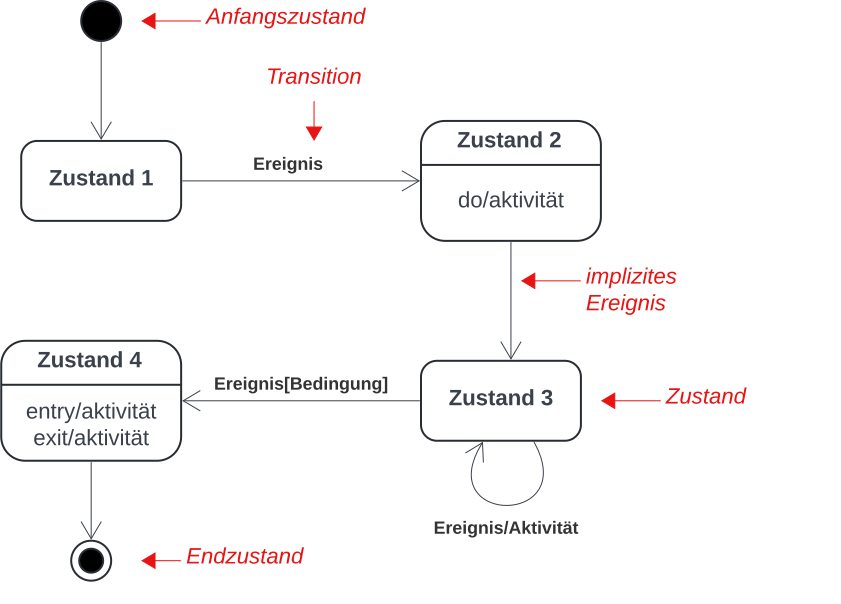
\includegraphics[scale=0.4]{part three/Zustandsautomaten/img/statechartdiagramnotation}
    \caption{Elemente eines einfachen Zustandsautomaten. Eine Transitionen wird durch ein \textbf{Ereignis} ausgelöst, das ein \textit{Signal}, ein \textit{Operationsaufruf} oder auch eine bestimmte \textit{Attributänderung} sein kann. (Quelle: in Anlehnung an \cite[90, Abb. 2.11-6]{Bal05})}
    \label{fig:statechartdiagramnotation}
\end{figure}



\noindent
Zustände können so lange andauern, wie es bspw. die Dauer einer Aufgabe erfordert: Die Dauer ist für die Modellierung von Zuständen und \textbf{Aktivitäten} (s.u.) nicht relevant (vgl.~\cite[88]{Bal05}). \\

\noindent
Sie beginnen mit dem Durchlaufen einer \textbf{Transition}, die zu dem Zustand hinführt, und enden mit dem Durchlaufen einer Transition, die von dem Zustand wegführt.\\
Innerhalb dieser Zeitspanne ist der Zustand aktiv.\\

\noindent
Ein Zustand kann \textbf{interne Aktivitäten} beinhalten (s. Abbildung~\ref{fig:entryexitdo}):

\begin{itemize}
    \item \textbf{Eintrittsaktivitäten} (\code{entry}): Wird ausgeführt, sobald sich das Objekt im betreffenden Zustand befindet.
    \item \textbf{Austrittsaktivitäten} (\code{exit}): Wird ausgeführt, bevor der Zustand verlassen wird.
    \item \textbf{andauernde Aktivitäten} (\code{do}): Wird ausgeführt, sobald ein Objekt den betreffenden Zustand einnimmt, und endet, sobald der Zustand verlassen wird.
    \item ein Zustand kann weitere interne Aktivitäten aufweisen (\cite[69]{Buh09})
\end{itemize}

\begin{figure}
    \centering
    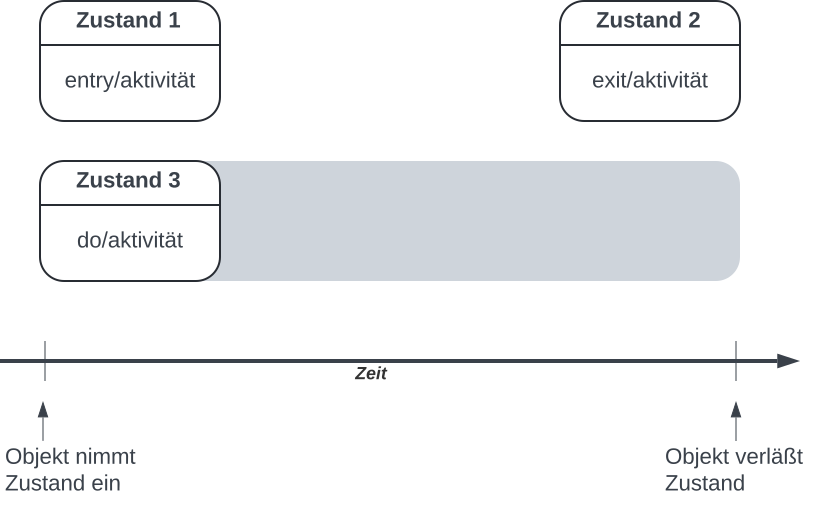
\includegraphics[scale=0.4]{part three/Zustandsautomaten/img/entryexitdo}
    \caption{Notationen für \textbf{entry}-,\textbf{exit}- und \textbf{do}-Aktivitäten sowie deren Dauer. Die \textbf{do}-Aktivität endet, wenn der Zustand verlassen wird. Die \textbf{entry}-Aktivität beendet sich von selbst. (Quelle: in Anlehnung an \cite[89, Abb. 2.11-3]{Bal05})}
    \label{fig:entryexitdo}
\end{figure}

\noindent
In der UML wird ein Zustand in einem Zustandsdiagramm als Rechteck mit abgerundeten Kanten dargestellt.\\

\noindent
\textbf{Start}- und \textbf{Endzustände} werden wie die in Abschnitt~\ref{sec:aktivitaetsdiagramme-begriffe-und-elemente} vorgestellten Start- und Endzustände dargestellt.


\subsection{Event und Transition}

\subsubsection*{Transition}
Eine \textbf{Transition} ist der \textit{Übergang} von einem Zustand zum nächsten (Ausgangs- / Folgezustand) und wird als gerichteter Graph dargestellt.\\

\noindent
Übergänge werden durch \textbf{Ereignisse} (\textit{Events}) ausgelöst.\\
Objekte können auf Events reagieren, oder diese ignorieren.\\

\noindent
Die \textbf{Signatur} einer Transition ist \code{Event[Guard]/Effekt} (\cite[321]{OMG17}).

\subsubsection*{Event (Ereignis)}
Transitionen werden durch Ereignisse ausgelöst (vgl.~\cite[91]{Bal05}).\\
Es werden folgende Arten von Events definiert (vgl.~\cite[69]{Buh09}):

\begin{itemize}
    \item \code{CallEvent}: Operationsaufruf; Der Ausgangszustand führt die Operation aus, und das Objekt wechselt in den Folgezustand.
    \item \code{SignalEvent}: Das Ereignis wird ausgelöst, wenn in einem (asynchronen) Prozess das Objekt dieses Signal empfängt.
    \item \code{ChangeEvent}: Ein Ereignis, das immer mit \code{when} beginnt und als boolescher Ausdruck notiert wird. Das Ereignis wird ausgelöst, wenn der Ausdruck von \code{false} zu \code{true} wechselt.
    \item \code{TimeEvent}: Definiert eine Zeitspanne, nach der das Ereignis ausgelöst wird.
    \item \code{AnyReceiveEvent}: Wird ausgeführt, wenn Ereignisse eintreffen, die nicht näher spezifiziert sind. Dieses Ereignis wird mit \code{all} beschriftet (vgl.\cite[293]{OMG17})\footnote{bei \textit{Balzert} wird das Ereignis \textit{AnyTrigger} erwähnt, das sich so in \cite{OMG17} nicht findet.}
\end{itemize}

\subsubsection*{Guard}
Ein \code{Guard} wird in eckigen Klammern als boolescher Ausdruck geschrieben.\\
Wenn der Ausdruck zu \code{true} wechselt, wird die Transition ausgeführt.

\begin{tcolorbox}
    Ein Guard ist nicht mit einem Change Event zu verwechseln:\\

    \blockquote[{\cite[292]{OMG17}}]{
        A ChangeEvent occurs when a Boolean \textcolor{blue}{changeExpression} becomes true. For example, this could be as a result of a
        change in the value of some Attribute or a change in the value referenced by a link corresponding to an Association. A
        ChangeEvent occurs implicitly and is not the result of any explicit action.
    }\\

    \noindent
    Ein \code{Guard} gibt an, unter welchen Bedingungen eine Transition stattfinden kann.\\
    Eine \code{ChangeEvent} wird unter bestimmten Bedingungen ausgelöst und führt damit zu einer Transition.
\end{tcolorbox}

\subsubsection*{Effekt (Aktivität)}
Ein \textbf{Effekt} (\textit{Aktivität}\footnote{\cite[88]{Bal05}}) definiert Aktionen, die \textit{während} einer Transition auszuführen sind (z.B. Neuberechnung eines Wertes aufgrund des geänderten Zustands).\\

\begin{tcolorbox}
    \textbf{Aktivitäten} sind mit einzelnen \textbf{Transitionen} verknüpft, \code{entry}/\code{exit}/\code{do}-Aktivitäten mit Zuständen: Diese werden immer ausgeführt, unabhängig von der Transition, die zu dem Zustand geführt hat.
\end{tcolorbox}

\subsubsection*{Entscheidung}
Soll eine Transition mittels Guards in mehrere überwachte Transitionen aufgeteilt werden, kann eine \textbf{Entscheidung} modelliert werden.
Die auszuführende Transition wird \textbf{dynamisch} (\textit{dynamic conditional branch}, s.~\cite[339 f.]{Bal05}) ausgewählt, wenn der Guard erreicht wird.

\subsubsection*{Terminator}
Ein \textbf{Terminator} (\textit{terminate pseudo state})(in der UML dargestellt als großes "X") ist ein \textbf{Pseudozustand}, den man verwenden kann, um auszudrücken, das Objekte dynamisch ``vernichtet`` werden können (vgl. ~\cite[341]{Bal05}): Der Unterschied zum \textbf{Endzustand} besteht hierbei, dass auch die Lebensdauer des betreffenden Objektes beendet wird. \textit{Balzert} ergänzt, dass es sich beim \textbf{Endzustand} \textit{nicht} um einen Pseudozustand, sondern um einen echten Zustand handelt.

\subsubsection*{Kreuzung}
\textbf{Kreuzungen} teilen eine oder mehrere eingehende Transition in eine oder mehrere ausgehende Transition auf.\\
Sind Guards vorhanden, werden diese \textbf{vor} der Kreuzung ausgewertet.
Im Gegensatz zu dem Entscheidungszustand handelt es sich um eine statische Verzweigung (\textit{static conditional branch}, s.~\cite[340]{Bal05}).\\
\textit{Buhl} merkt an, dass mit Hilfe von Kreuzungen Automaten übersichtlicher werden (vgl.~\cite[73]{Buh09}).


\subsubsection*{Zusammengesetzte Zustände}
Hierarchien von Zuständen können modelliert werden, indem \textbf{zusammengesetzte Zustände} verwendet werden, die sich aus \textbf{Unterzuständen} zusammensetzen.\\

\noindent
Beim Betreten von zusammengesetzten Zuständen können mehrere Arten unterschieden werden. \textit{Buhl} führt wie folgt auf (vgl.~\cite[73]{Buh09}):

\begin{itemize}
    \item \textbf{Standardeintritt}: Transition führt zum Rand des zusammengesetzten Zustands, wodurch der darin enthaltene Startzustand aktiviert wird
    \item \textbf{expliziter Eintritt}: Transition führt zu einem Zustand im zusammengesetzten Zustand
    \item \textbf{flache Historie} (\textit{shallow history}): speichert den letzten Zustand in einem Unterzustand
    \item \textbf{tiefe Historie} (\textit{deep history}): speichert den letzten Zustand im Unterzustand und auch die Zustände der tiefer liegenden Unterzustände
    \item \textbf{Eintrittspunkt}: Transitionen enden am Eintrittspunkt und werden dann neu erzeugt, und enden an einem weiteren zusammengesetzten Zustand oder einem einfachen Zustand
\end{itemize}

\noindent
Beim Verlassen von Zuständen können ebenfalls mehrere Arten verwendet werden:

\begin{itemize}
    \item \textbf{Endzustand}: der zusammengesetzte Zustand wird beendet.
    \item \textbf{Terminator}: der gesamte \textit{Automat} wird beendet.
    \item \textbf{Transition aus einem inneren Zustand}: die Transition führt von einem Zustand aus dem zusammengesetzten Zustand heraus
    \item \textbf{Transition aus einem zusammengesetzten Zustand}: die Transition wird an den zusammengesetzten Zustand angetragen und führt heraus
    \item \textbf{Austrittspunkt}: eine Transition führt zum Ausgangspunkt und der zusammengesetzte Zustand wird verlassen, im Anschluss wird die vom Austrittspunkt wegführende Transition ausgeführt
\end{itemize}


\begin{tcolorbox}[colback=yellow!20]
\cite[Abb. 6.11.7, 342]{Bal05}: tiefe Historie. Z3 außerdem als Beispiel, dass Zustände interne Zustände besitzen können,
\end{tcolorbox}

\subsubsection*{Regionen}
\textbf{Regionen} dienen zur Darstellung paralleler oder konkurrierender Abläufe in einem Zustandsautomaten: Hier gelten ebenso alle Aussagen über Zustände


\begin{tcolorbox}[colback=yellow!20]
    Beispiel Radio für Regionen.
\end{tcolorbox}

\subsection{Implementierung}
Zustandsautomaten werden klassischerweise mit einer \code{switch}-Anweisung realisiert: Einzelne Zustände werden als Konstanten abgelegt, die die \code{switch}-Anweisung steuern.\\
Verschiedene Operationen realisieren dann die \code{do}-, \code{entry}- und \code{exit}-Aktionen sowie die Effekte der Zustände sowie die Rückgabe der Folgezustände (vgl. \cite[75]{Buh09}).